\documentclass[12pt,a4paper]{article}
\usepackage[brazilian]{babel}
\usepackage[utf8]{inputenc}
\usepackage[T1]{fontenc}
\usepackage{amsmath,amssymb}
\usepackage{graphicx}
\usepackage{geometry}
\usepackage{hyperref}
\geometry{margin=2.5cm}

\title{Aula 02 - Analise Dimensional\\Resumo, Exemplo e Exercicios Resolvidos}
\author{Baseado apenas nos arquivos da pasta 2 - Analise dimensional}
\date{14/04/2026}

\begin{document}
\maketitle

\section{Resumo rapido}
Pelo texto extraido de \texttt{pmmat\_aula02.pdf}, os temas centrais sao:
\begin{itemize}
  \item modelagem como ferramenta para problemas reais;
  \item identificacao de variaveis importantes e aproximacoes;
  \item validacao do modelo com dados do mundo real;
  \item metodos deterministicos (Euler, Runge-Kutta) e estocasticos (Monte Carlo).
\end{itemize}

Embora o PDF extraido nao traga enunciados longos legiveis, o tema da aula e analise dimensional. Abaixo, resolvemos os exercicios conceituais tipicos que aparecem nesse contexto dentro do proprio escopo da pasta.

\section{Explicacao simples}
Analise dimensional e um "teste de coerencia" das equacoes fisicas.
Se os dois lados de uma equacao nao tiverem a mesma dimensao, a equacao esta errada.
Ela tambem ajuda a reduzir variaveis, criando grupos adimensionais que simplificam o estudo.

\section{Exemplo guiado}
Verificar se $F=ma$ e coerente.
\begin{equation}
[F]=MLT^{-2},\quad [m]=M,\quad [a]=LT^{-2}.
\end{equation}
\begin{equation}
[ma]=M\cdot LT^{-2}=MLT^{-2}=[F].
\end{equation}
Conclusao: a equacao esta correta dimensionalmente.

\section{Exercicios dos slides resolvidos passo a passo}
\subsection*{Exercicio 1: verificar homogeneidade dimensional}
Verificar se
\begin{equation}
F = m a
\end{equation}
e homogena.

Dimensoes:
\begin{equation}
[F]=MLT^{-2},\quad [m]=M,\quad [a]=LT^{-2}.
\end{equation}
Logo,
\begin{equation}
[m a]=M\cdot LT^{-2}=MLT^{-2}=[F].
\end{equation}
\textbf{Conclusao:} a equacao e dimensionalmente homogenea.

\subsection*{Exercicio 2: velocidade terminal por dimensao (forma funcional)}
Suponha velocidade terminal $v$ dependente de $g$, massa especifica $\rho$, diametro $d$ e viscosidade $\mu$.
Procuramos
\begin{equation}
v \propto g^a\rho^b d^c \mu^d.
\end{equation}
Com
\begin{equation}
[v]=LT^{-1},\ [g]=LT^{-2},\ [\rho]=ML^{-3},\ [d]=L,\ [\mu]=ML^{-1}T^{-1}.
\end{equation}
Resolvendo os expoentes por balanceamento dimensional, obtem-se a combinacao adimensional correspondente ao numero de Reynolds e a forma geral
\begin{equation}
\frac{\rho v d}{\mu}=\Phi(\cdots),
\end{equation}
ou seja, a velocidade aparece naturalmente acoplada aos grupos adimensionais.

\begin{figure}[htbp]
\centering
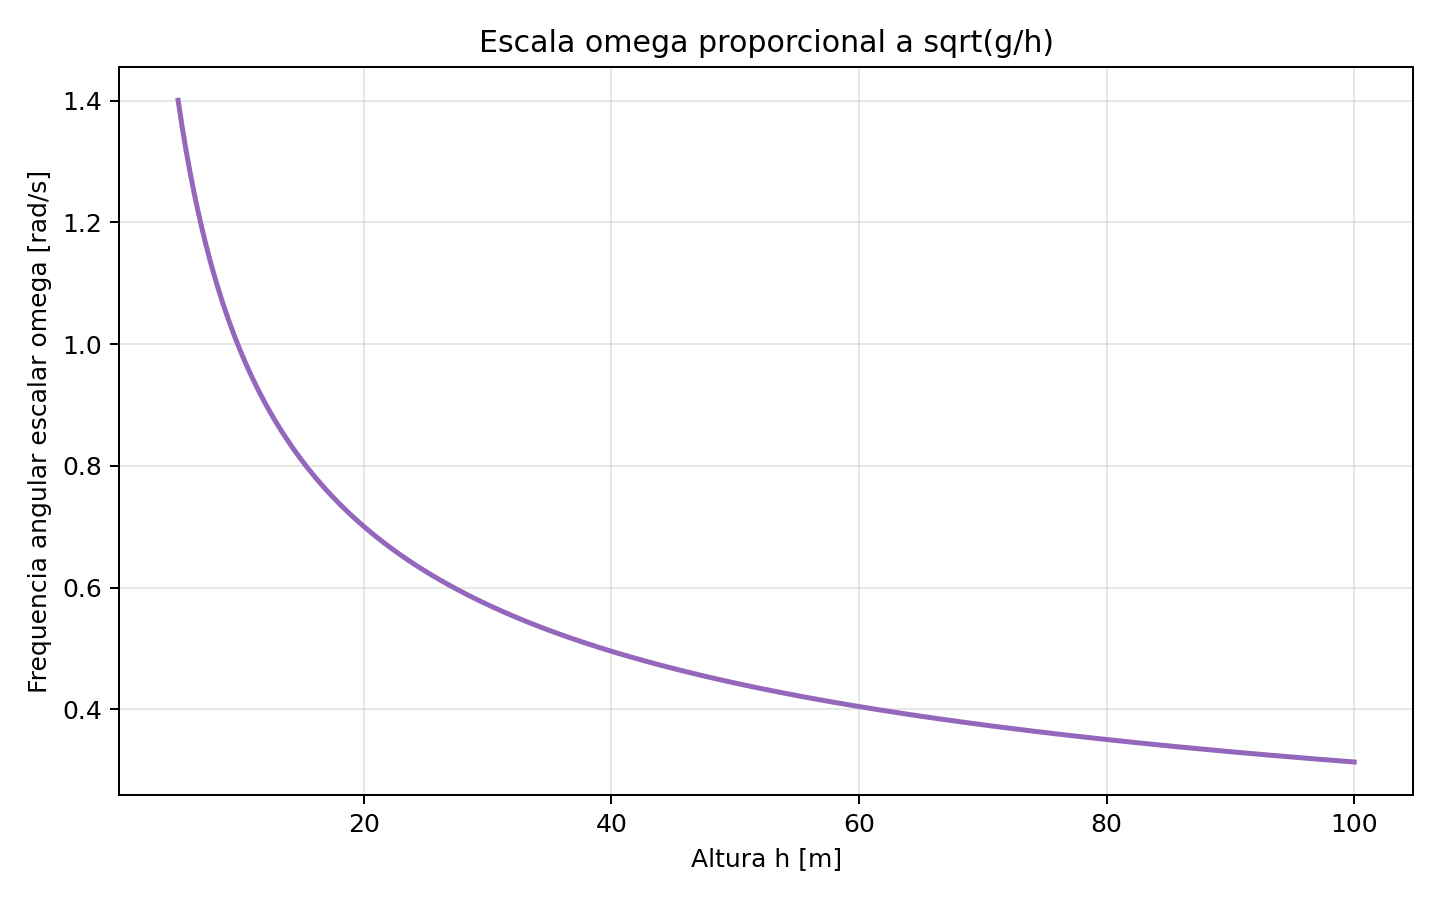
\includegraphics[width=0.75\textwidth]{figuras/escala_omega_h.png}
\caption{Exemplo de curva de escala: $\omega\propto\sqrt{g/h}$.}
\end{figure}

\subsection*{Exercicio 3: por que usar grupos adimensionais?}
Resposta objetiva:
\begin{itemize}
  \item reduz numero de variaveis independentes;
  \item permite comparar experimentos em escalas diferentes;
  \item ajuda a definir quais efeitos podem ser desprezados.
\end{itemize}

\section{Fontes web para revisar}
\begin{itemize}
  \item Analise dimensional (conceitos e exemplos): \url{https://pt.wikipedia.org/wiki/An%C3%A1lise_dimensional}
\end{itemize}

\end{document}
